\documentclass[main.tex]{subfiles}
\begin{document}
    
\chapter{Safety}
\label{ch:safety}
\section{Embedded \& Communication Systems}
\subsection{Pre-launch Tests}
\begin{table}[H]
	\centering
	\begin{tabular}{@{}lll@{}} \toprule
    Sub-System & Test Description & Nominal Values \\ \midrule
    Motor & Nominal Current Draw at ESC & \\
    Motor & Nominal Temperature MOTOR & \\
    Motor & Nominal Temperature ESC & \\
    Motor & Cooling pump is active, cooling pressure less than & $< \SI{14.5}{psi}$ \\
    Friction & Pressure sensor & $< \SI{250}{psi}$ \\
    Friction & Solenoid control to turn on and off & TRUE \\
    Batteries & Nominal Voltage and Current Main Battery & \\
    Batteries & Nominal Temperature Main Battery & $20 < \textrm{Temp} < 50$ \\
    Batteries & Nominal Voltage and Current 24V Battery & 24 volts \\
    Batteries & Nominal Temperature 24V Battery & $20 < \textrm{Temp} < 50$ \\
   	Batteries & Nominal Voltage from 25V to 5V step-down & 5 volts \\
    Navigation & IMUs are functional and give normal values  & \SI{0}{m/s} acceleration \\
    Navigation & Shaft Encoder at \SI{0}{rpm} and Functional & Drive Test \\
    Navigation & Tilt sensors nominal values and online & $< 10 ^\circ$ \\
    Navigation & Test Navigation system working (drive 1 meter) & Output 1 meter \\
    Navigation & ESC output is nominal & Drive Test \\
    EC-Brakes & Reed sensor state & \\
    EC-Brakes & Nominal Temperature & \\
    EC-Brakes & Solenoid Controls online & \\
    Other & Photoelectric distance is Nominal & \\ \bottomrule
    \end{tabular}
	\caption{Pre-Launch Self-Checks. Will be ran on pod before any launch. Described as System Health Check in pod state diagram \reffig{fig:pod-failure-state-diagram}}
    \label{tlb:prelaunch-tests}
\end{table}

    \subsection{Heartbeat}
    There are going to be three types of heartbeats in the system:
    \begin{itemize}
      \item Master-machine $\rightarrow$ Control-panel Heartbeat
      \item Hub $\rightarrow$ Master-machine Heartbeat
      \item Sensor $\rightarrow$ Hub Heartbeat
    \end{itemize}
    
    In case of any of the heartbeat failing, the master that is being reported to, is capable of restarting a slave i.e. triggering the watchdog procedure.
    
	\subsection{Watchdogs}
    With two types of machines used in the pod's Embedded-systems, ATMega and RPI, each one has a different approach to Watchdogs. Arduino has a built in Watchdog that can be configured and with it's non-volatile memory, a lot of the state information can be preserved and recovered after a reboot. RPI has an OS-level Watchdog as well, but having a much more complex OS to load, reboots will take longer. Exact number will be generated through a series of tests.
   
    \subsection{Single points of failure}
    
    
    \subsection {Failure scenarios and state diagram}
    
  In the event of pod failures, the control system will respond accordingly to ensure no harm is caused to the pod, the team, the test track, or the environment. If a system fails, the pod is designed to ensure it is just as safe as when it was operating correctly.\\
  The following table below lists the failure modes and effects according to specific failure scenarios. The software failure scenarios include, but are not limited to: the main battery, embedded system, braking, navigation, friction drive, and sensors.
  The software failure state diagram \reffig{fig:pod-failure-state-diagram} shows the behaviour and flow of the control systems. In addition, \reftab{tlb:fail-table} shows all of the possible failure scenarios and according software actions that are taken as a consequence.\\
  
\begin{table}[p]
\centering
\begin{tabular}{@{}p{3cm}p{13cm}@{}}
\toprule 
 Source & Action\\
\midrule
Main Battery dies or fails & EC brakes engage based on circuit design, provide power to friction brakes if speed is less than \SI{10}{m/s}\\
% \hline
Server side power wire is down& Case 1: One server dies, switch to the next server; Case 2: All servers die, Embedded loses heartbeat\\
% \hline
Embedded subsystem dies& Active server will ground the pod\\
% \hline
Friction subsystem dies& Activate braking, cut off power to motor\\
% \hline 
Braking subsystem dies& Keep navigation active; Keep safety mechanisms on; Shut down other systems\\
% \hline
Navigation subsystem dies& Brakes: Keep braking; Acceleration: Cut off acceleration, activate EC/friction brakes; If speed is greater than 10 m/s, do not activate friction\\
% \hline 
Brakes overheat& Braking: Keep braking (Friction and EC brakes); Acceleration: Cut off acceleration, activate EC/Friction brakes\\
% \hline
24V battery dies or fails&Case 1: 1 battery dies: Brakes engage; Provide power to friction drive if speed is less than 10 m/s; Case 2: both batteries die:  Lose all 3 servers, Embedded loses heartbeat; Brakes engage\\
% \hline
Friction drive slips on the rail&Use a filter if there is a spike (non-linear slope); If friction drive slips for less than 0.5 seconds, cut friction, stop accelerating; If 0.5 seconds or more, cut power and gradually increase to the original target; Else, check ESC reaction time and cut off power\\
% \hline 
Computer overheats & Shut down server\\
% \hline
Shortings, Current too high & Shut down associated battery; start braking\\
% \hline 
Temperature sensor malfunction & If 2/3 sensors are consistent, ignore the remaining 1/3 sensors\\
% \hline
Voltage / Current sensor malfunction& If voltage or current sensors outside of tolerance, engage braking\\
% \hline 
Photoelectric Distance sensor malfunction& If 1/4 sensors outside of tolerance or zero, ignore and read the remaining 3/4 sensors; If 2/4 sensors are wrong: refer to IMU regarding gyroscope\\
% \hline
Acceleration sensor malfunction& If 1 sensor is wrong: ignore and read remaining sensor; Else: shutdown\\
% \hline 
Tilt sensor malfunction & Refer to IMU. If IMU is consistent with tilt sensor, brake \\
% \hline
RPM Sensor/ Shaft encoder malfunction & Refer to IMU for acceleration data \\
% \hline 
Reed Sensor malfunction & Refer to IMU for deceleration data \\
\bottomrule
\end{tabular}
\caption{Software Failure Scenarios}
\label{tlb:fail-table}
\end{table}

\begin{figure}
  \centering
  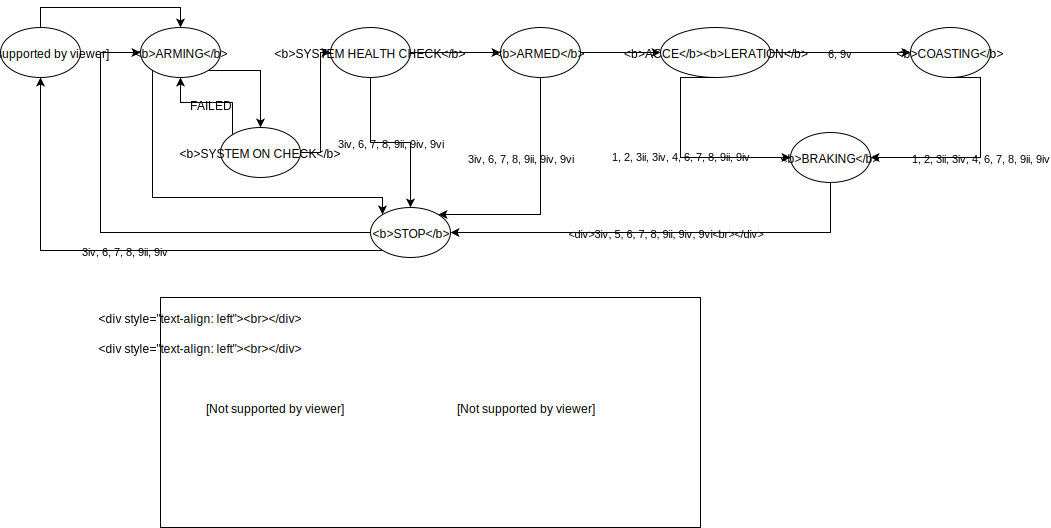
\includegraphics[width=\textwidth]{images/Pod_Failure_Diagram.png}
  \caption{ Pod Failure State Diagram}
  \label{fig:pod-failure-state-diagram}
\end{figure}

    \subsection{Tests \& Validation}
    \begin{itemize}
    \item \textbf{Vacuum Test.} All of the electrical components located on-board of the pod (such as MEB, HPB). While RPIs and ATMega has been tested in a vacuum chamber last year, it is important to test functionality of the entire system, since significant changes have been made. Important points of observation is the machine (RPI and Arduino) and sensor (for a complete sensor list refer to \reffig{tab:pod-sensor-list}) temperature. 
    \item \textbf{Independent Sensor Test.} Validate functionality of all sourced components. Confirm sensor refresh rate and optimal mounting positions.
    \item \textbf{Navigation system test.} Series of HiL tests to simulate pod movement and Unit-test software elements. drive pod without power and measure navigation. Then drive pod with power and measure navigation again
    \item \textbf{Communication System Test.} Stress test entire communication pipeline from sensors to Control-Panel. Goal of test is to find at what network load, the data transfer rate slows down to an unsafe conditions.
    \item \textbf{System / Sub-components Power Loss} Test complete system power loss scenario as well as partial sub-system power loss.
    \item \textbf{Watchdog reload time} Test how long it takes to reload a Master-machine as well as a Hub with OS provided watchdog.
    \end{itemize}
    
\begin{table}[p]
\centering
\begin{tabular}{@{}p{3cm}p{13cm}@{}}
  \toprule 
	
  \bottomrule
\end{tabular}
\caption{Software Failure Scenarios}
\label{tlb:fail-table}
\end{table}
    
   
\end{document}